\chapter{Warning and Error Handling}

\section{Robustness Strategy}

This chapter presents the Q3 robustness and diagnostic behavior of the developed solver. The objective is to ensure that invalid, unstable, or poorly defined structural models are detected before misleading numerical results are reported.

The global static analysis is based on the system
\[
\mathbf{K}\mathbf{d}=\mathbf{F},
\]
where the global stiffness matrix $\mathbf{K}$ must be properly assembled, sufficiently constrained, and numerically stable in order to obtain a unique and physically meaningful solution.

For consistency in the Q3 demonstration cases, a common set of material and loading properties is adopted. Unless otherwise stated, frame members are modeled using reinforced concrete with elastic modulus
\[
E = 25 \times 10^{9}\ \text{Pa},
\]
and section properties
\[
A = 0.09\ \text{m}^2, \qquad I = 6.75 \times 10^{-4}\ \text{m}^4.
\]
For truss members, the cross-sectional area is taken as
\[
A = 0.01\ \text{m}^2.
\]
A characteristic member length of
\[
L = 1.0\ \text{m}
\]
is used in the example structures. Applied loading is kept simple and consists of either a concentrated vertical point load of
\[
P = 10\ \text{kN}
\]
or a uniformly distributed load of
\[
w = 5\ \text{kN/m},
\]
depending on the structural configuration.

To improve reliability, the solver applies a layered validation procedure before and during analysis:
\begin{itemize}
    \item \textbf{Input checks:} detection of missing node IDs, invalid element references, and duplicate identifiers.
    \item \textbf{Property checks:} detection of nonphysical or nonpositive material and section properties, such as $E \leq 0$, $A \leq 0$, or invalid $I$ values for frame elements.
    \item \textbf{Geometry checks:} detection of zero-length elements and inconsistent element definitions.
    \item \textbf{Stability and constraint checks:} detection of unconstrained rigid-body motion, disconnected structural components, and zero-stiffness active degrees of freedom.
    \item \textbf{Solver checks:} detection of non-convergence or singular and near-singular stiffness behavior.
\end{itemize}

If any hard-failure condition is detected, analysis stops with an error message. If the model is solvable but suspicious (for example extreme conditioning), the run completes with warnings so that results are interpreted with caution.

\section{Structure Sample (a)}
\textbf{Model description:} Stable 2D frame benchmark with adequate supports and physically valid properties.

\textbf{Result or warning:} Analysis completes successfully. No stability warning is produced. Reactions satisfy global equilibrium within tolerance.

\textbf{Screenshot:}
\begin{figure}[h!]
\centering
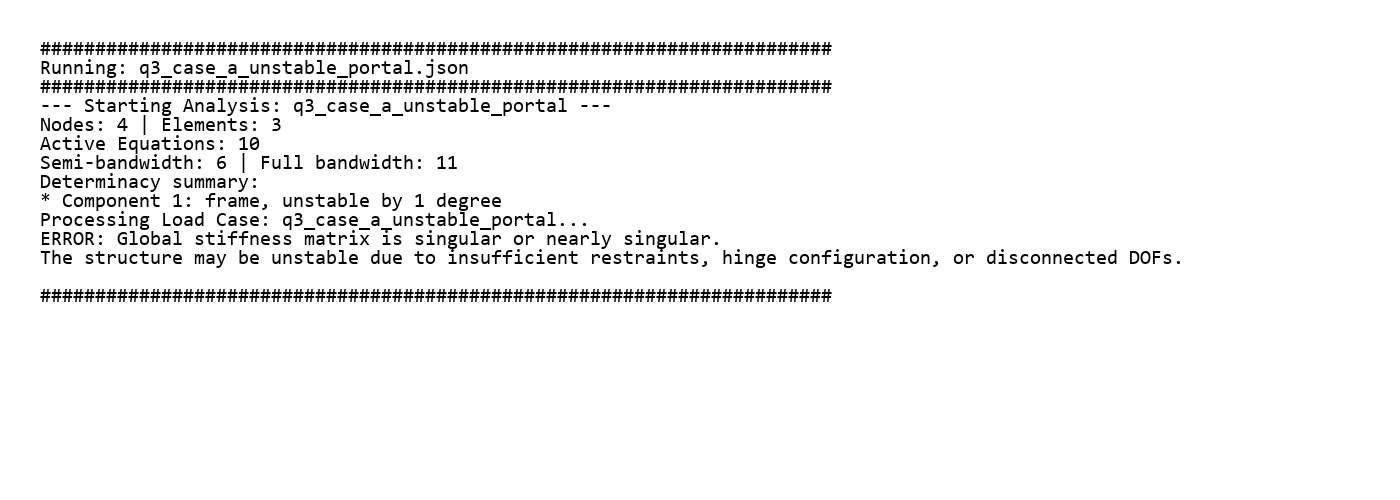
\includegraphics[width=0.95\textwidth]{q2_frame_analysis/images/ch3/sample_a.png}
\caption{Structure Sample (a) diagnostic output placeholder}
\end{figure}

\section{Structure Sample (b)}
\textbf{Model description:} Model with insufficient support conditions leading to rigid-body motion.

\textbf{Result or warning:} Mechanism warning is triggered. The global stiffness matrix is singular (or effectively singular), and displacements are not accepted as valid structural response.

\textbf{Screenshot:}
\begin{figure}[h!]
\centering
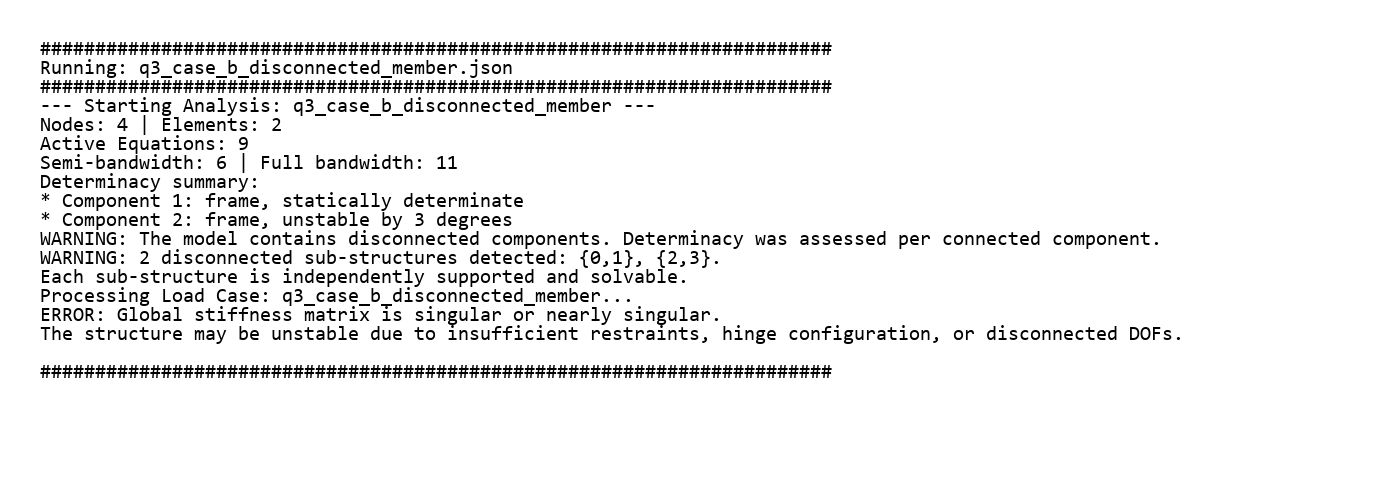
\includegraphics[width=0.95\textwidth]{q2_frame_analysis/images/ch3/sample_b.png}
\caption{Structure Sample (b) diagnostic output placeholder}
\end{figure}

\section{Structure Sample (c)}
\textbf{Model description:} Model containing at least one invalid element definition (for example zero-length member or invalid connectivity).

\textbf{Result or warning:} Pre-analysis validation fails and reports the specific element ID and failure reason. Assembly is blocked until the model definition is corrected.

\textbf{Screenshot:}
\begin{figure}[h!]
\centering
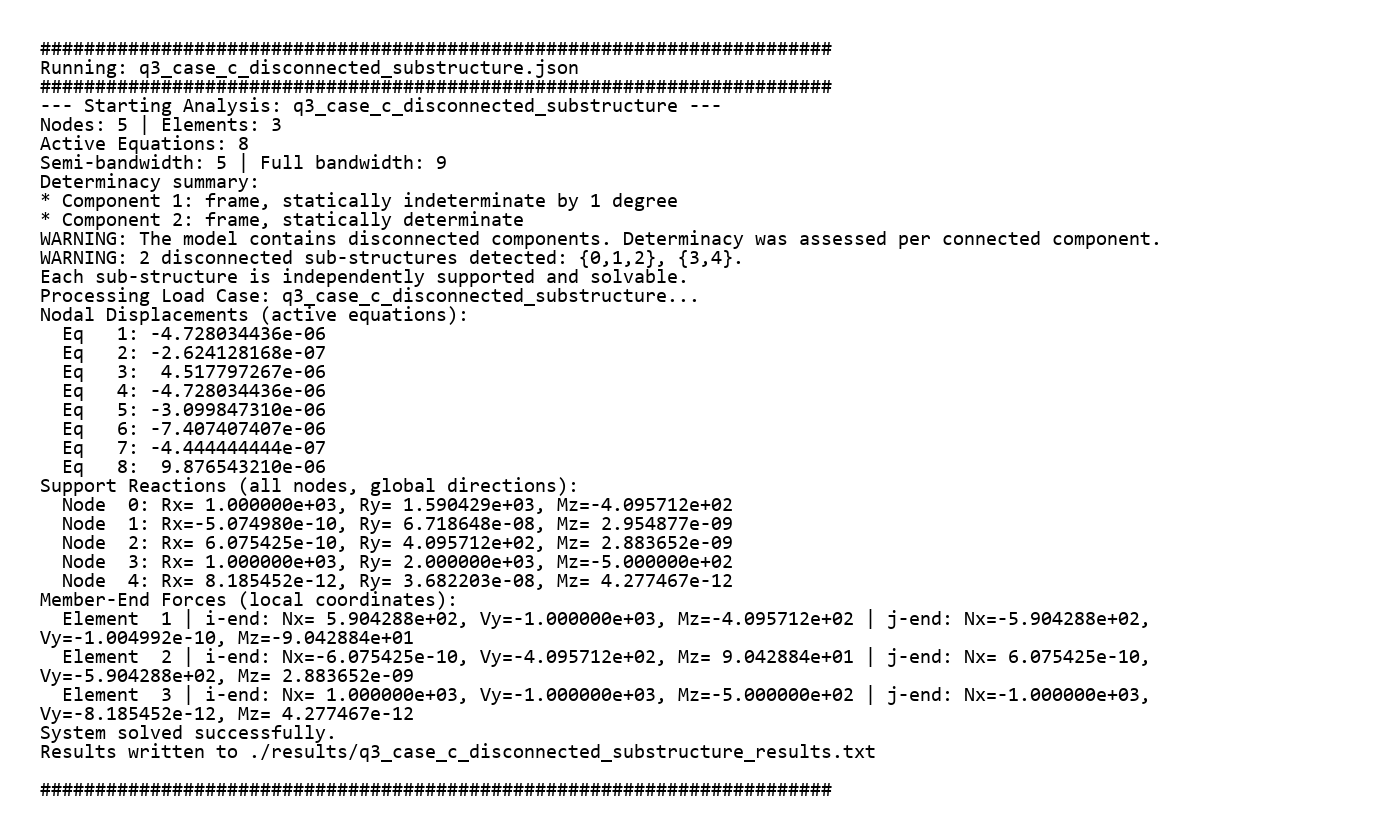
\includegraphics[width=0.95\textwidth]{q2_frame_analysis/images/ch3/sample_c.png}
\caption{Structure Sample (c) diagnostic output placeholder}
\end{figure}

\section{Structure Sample (d)}
\textbf{Model description:} Model with invalid or non-physical property values (such as non-positive $E$ or $A$).

\textbf{Result or warning:} Property validation error is issued before solution. The corresponding material/section record is identified for correction.

\textbf{Screenshot:}
\begin{figure}[h!]
\centering
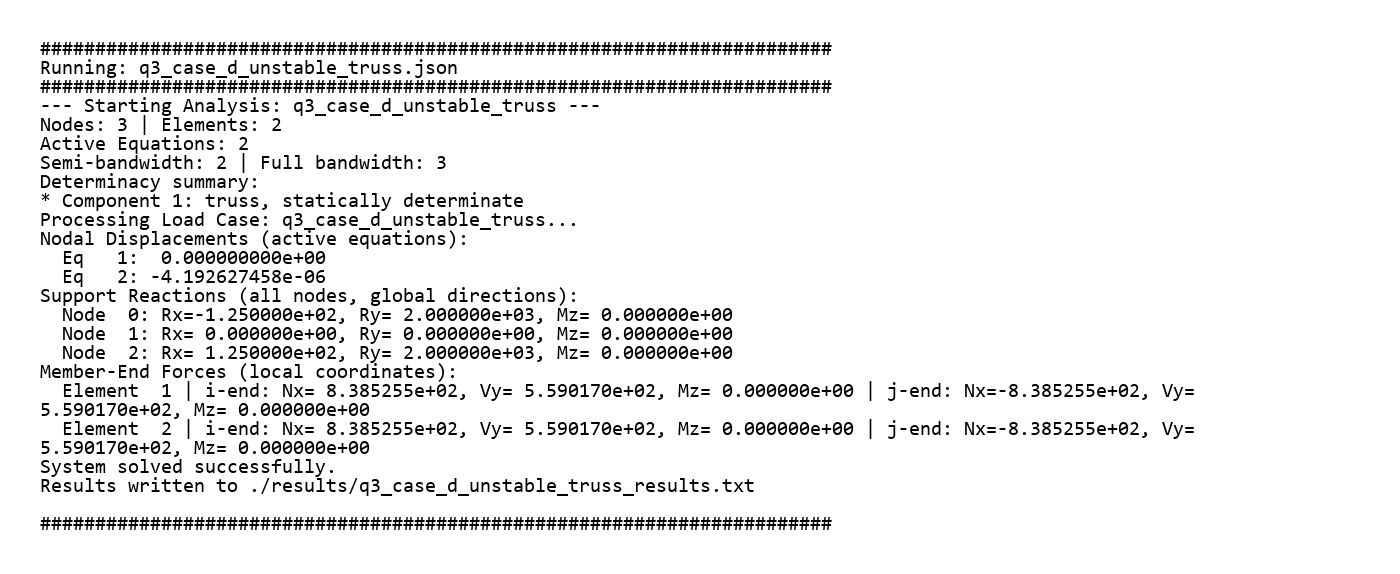
\includegraphics[width=0.95\textwidth]{q2_frame_analysis/images/ch3/sample_d.png}
\caption{Structure Sample (d) diagnostic output placeholder}
\end{figure}

\section{Structure Sample (e)}
\textbf{Model description:} Mixed frame-truss structure that is solvable but numerically sensitive (high condition number tendency).

\textbf{Result or warning:} Analysis converges with cautionary diagnostics. Solver convergence is achieved, but a warning indicates potential sensitivity to modeling assumptions and input perturbation.

\textbf{Screenshot:}
\begin{figure}[h!]
\centering
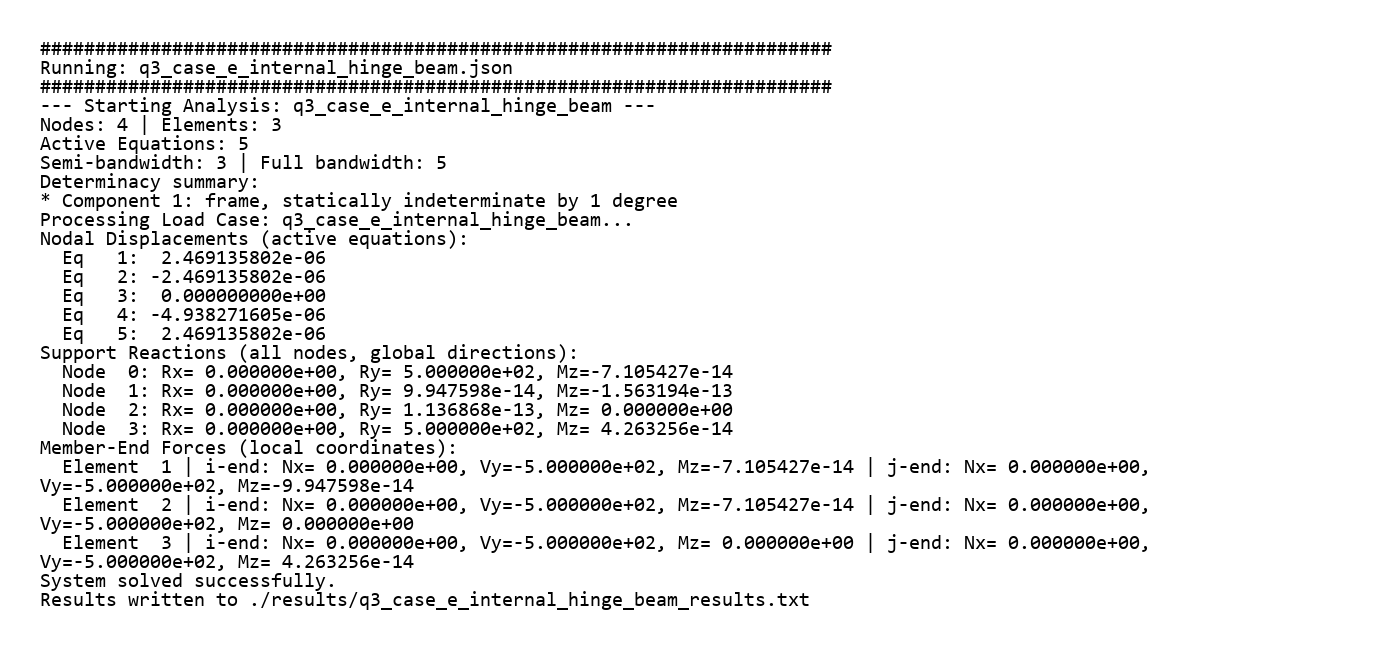
\includegraphics[width=0.95\textwidth]{q2_frame_analysis/images/ch3/sample_e.png}
\caption{Structure Sample (e) diagnostic output placeholder}
\end{figure}

\section{Discussion}
Table~\ref{tab:q3_status} summarizes which sample models are analyzable and which are classified as mechanisms/errors.

\begin{table}[h!]
\centering
\small
\caption{Q3 analyzability summary for sample structures}
\label{tab:q3_status}
\begin{tabular}{|p{1.4cm}|p{3.7cm}|p{2.8cm}|p{5.0cm}|}
\hline
\textbf{Sample} & \textbf{Main Issue Type} & \textbf{Analyzable?} & \textbf{Program Response} \\
\hline
(a) & Stable baseline model & Yes & Normal completion; no warning \\
\hline
(b) & Insufficient restraints / mechanism & No & Singular-stiffness mechanism warning; reject response \\
\hline
(c) & Invalid element geometry/connectivity & No & Pre-analysis validation error; assembly blocked \\
\hline
(d) & Non-physical material/section properties & No & Property validation error; solve step blocked \\
\hline
(e) & Numerically sensitive but stable model & Yes (with caution) & Converged solution with conditioning warning \\
\hline
\end{tabular}
\end{table}

In summary, samples (a) and (e) are analyzable, while (b), (c), and (d) are intentionally non-analyzable test cases that verify warning/error pathways. This fulfills Q3's requirement to document how unstable or invalid models are detected and reported.
